% !TEX root = /media/ueslei/Ueslei/INPE/PCI/Guia_COAWST/main.tex
\chapterimage{ocean2.jpg} % Chapter heading image
\chapter{Introdução}

\bigskip

%%%%%%%%%%%%%%%%%% ROMS %%%%%%%%%%%%%%%%%%%%

\section{O Regional Ocean Modeling System}\index{Regional Ocean Modeling System}
\bigskip
\noindent O Regional Ocean Modeling System (ROMS; \cite{Shchepetkin2005}) é um modelo oceânico tridimensional de superfície livre, coordenada vertical sigma (que segue o terreno) e resolve equações primitivas. Este modelo utiliza a média de Reynolds e o método de diferenças finitas para resolver as equações de Navier-Stokes assumindo aproximações hidrostáticas e de Boussinesq (\cite{Haidvogel2008}).
\bigskip

\noindent As equações hidrostáticas de momentum utilizam um esquema de passo de tempo \textit{split-explicit}, aonde os modos barotrópico e baroclínico são resolvidos separadamente em distintos números finitos de passos de tempo para resolver as equações de superfície livre e momentum integrado na vertical. A estrutura de passos de tempo separados mantém a conservação de volume e a preservação de consistência que são necessárias para as equações de traçadores (\cite{Shchepetkin2005,Haidvogel2008}).
\bigskip

\noindent A partir da grade, o modelo resolve as equações na horizontal através de coordenadas curvilíneas ortogonais do tipo Arakawa-C (\cite{Arakawa1977}). Na vertical, as coordenadas seguem as feições do terreno e permitem ajustar a resolução ao longo da coluna d'água. Para garantir a conservação de momentum, a grade utiliza diferenças finitas de segunda ordem (\cite{Haidvogel2008}).
\bigskip

\noindent Segundo \textcite{Gouveia2015}, o ROMS está estruturado por diversos modulos escritos em liguagem em Fortran (\textit{.F}). Além deles também tem os arquivos de entrada (\textit{.in}) que contém as parametrizações numéricas do modelo, arquivos de cabeçalho (\textit{.h}) que fornecem informações de pré-processamento, arquivos com definições de variáveis (\textit{varinfo.dat}) e pelo \textit{makefile} usado para compilar os executáveis.
\bigskip

\noindent O ROMS é um modelo que possui códigos livre e seu desenvolvimento conta com a contribuição da comunidade de usuários. Atualmente, a versão utilizado no COAWST é gerenciado pelo Dr Hernan Arango da Rutgers University. Para acessar ao código do modelo, é necessário fazer o cadastro no site do ROMS (\textcolor{bleu_cite}{\textit{https://www.myroms.org/}}) para ter acesso ao código fonte do modelo. É necessário apresentar uma justificativa para se cadastrar no site. O site também conta com um fórum extremamente útil e bastante ativo (\textcolor{bleu_cite}{\textit{https://www.myroms.org/forum/}}) para perguntas e sugestões sobre problemas na utilização deste modelo.
\bigskip

%%%%%%%%%%%%%%%%%%%% WRF %%%%%%%%%%%%%%%%%%%%

\section{O Weather Research \& Forecasting Model}\index{Weather Research \& Forecasting Model}
\bigskip

\noindent O Weather Research and Forecasting (WRF; \cite{Skamarock2008}) é um modelo desenvolvido pelo National Centers for Environmental Prediction (NCEP), National Center for Atmospheric Research (NCAR) e grupos de pesquisa de diferentes universidades (\textcolor{bleu_cite}{\textit{https://www.mmm.ucar.edu/weather-research-and-forecasting-model}}).
\bigskip

\noindent Para integrar no tempo as equações governantes, o ARW utiliza modos de baixa freqüência que são integrados utilizando o esquema de Runge-Kutta de terceira ordem, e os modos acústicos (de alta frequência) integrados com passo de tempo menor, para manter a estabilidade numérica, através de um esquema “forward-backward” para os modos acústicos que se propagam horizontalmente, e de um esquema implícito para modos acústicos de propagação vertical e oscilações de empuxo (\cite{Skamarock2008}).
\bigskip

\noindent O modelo WRF utiliza uma grade do tipo Arakawa-C (\cite{Arakawa1977}). Nesta grade as velocidades normais estão escalonadas a meio comprimento da grade das variáveis termodinâmicas, conforme visualizado na Figura \textcolor{bleu_cite}{\ref{gradeswrf}}.
\bigskip


\begin{figure}[H]
    \centering
    \captionsetup{justification=centering}
    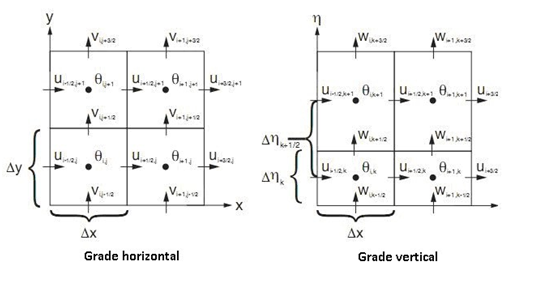
\includegraphics[width=0.80\textwidth]{grid.png}
    \centering \caption{Grade horizontal e vertical do Weather Research and Forecast (WRF) em Arawaka-C. \newline Fonte: \textcite{Skamarock2008}.}
    \label{gradeswrf}
\end{figure}
\bigskip

\noindent É importante ressaltar que o WRF, sem o acoplamento com outros modelos, simula a rugosidade da superfície baseada na Relação de rugosidade com o estresse do vento proposta por \textcite{Charnock1955}, como exemplificado na Equação \textcolor{bleu_cite}{\ref{equacao1}}:
\bigskip

\begin{equation}
Z_{0} = Z_{ch} \frac{u_{*}^{2}}{g}
\label{equacao1}
\end{equation}

\bigskip

\noindent Onde \textit{Z\textsubscript{0}} é a rugosidade, \textit{Z\textsubscript{ch}} é o parâmetro de Charnock (um valor adimensional de 0,018), \textit{U\textsubscript{*}} a velocidade de fricção (m/s) e \textit{g} a acerelação da gravidade (9,81 m/s\textsuperscript{2}).
\bigskip

%%%%%%%%%%%%%%%%%%% SWAN %%%%%%%%%%%%%%%%

\section{O Simulating Waves Nearshore}\index{Simulating Waves Nearshore}
\bigskip

\noindent O Simulating Waves Nearshore (SWAN; \cite{Booij1999,Booij1996}) é um modelo de terceira geração, concebido para simular ondas em águas rasas. Ele é fundamentado na equação espectral discreta do balanço da ação da onda. É amplamente utilizado na previsão numérica do espectro de ondas em regiões costeiras, estuários, canais e outros, podendo utilizar campos de vento, batimetria e correntes fornecidos por outros modelos \parencite{Booij1999,Booij1996}.
\bigskip

\noindent \textcite{Dasilva2013} e \textcite{Booij1999,Booij1996} elencam as principais características do SWAN:
\bigskip

\begin{itemize}
\item Refração de onda com profundidade variável;
\item Empinamento induzido pela profundidade e corrente;
\item Geração de ondas pelo vento;
\item dissipação por \textit{whitecapping};
\item Dissipação pela quebra de ondas induzida pela profundidade;
\item Dissipação devido à fricção com o fundo;
\item Interações não lineares de 3 e 4 ondas;
\item Difração.
\end{itemize}
\bigskip

%%%%%%%%%%%%%%%%%%% MCT %%%%%%%%%%%%%%%%
\section{O Model Coupling Toolkit}\index{Model Coupling Toolkit}
\bigskip

\noindent O Model Coupling Toolkip (MCT; \cite{Larson2005,Jacob2005,Warner2008}) é um conjunto de rotinas livres, escritas basicamente em Fortran 90 que são utilizadas no acoplamento de modelos. Ele é uma ferramenta muito poderosa pois permite que os modelos sejam acoplados também de forma paralela.
\bigskip

\noindent Segundo o site do MCT (\textcolor{bleu_cite}{\textit{http://www.mcs.anl.gov/research/projects/mct/}}), ele fornece os seguintes serviços de acoplamento de núcleo:
\bigskip

\begin{itemize}
\item Um registro das componentes dos modelos;
\item Descritores de decomposição do domínio;
\item Ferramentas paralelizadas para interpolação \textit{intergrid};
\item Ferramentas para mesclar dados de entre vários componentes;
\item Um modelo de programação semelhante ao MPI (Message Passing Interface).
\end{itemize}
\bigskip

%%%%%%%%%%%%%%%%%%%%% SCRIP %%%%%%%%%%%%%%
\section{ O Spherical Coordinate Remapping Interpolation Package}\label{scripsecao}
\bigskip

\noindent O  Spherical Coordinate Remapping Interpolation Package (SCRIP; \cite{Jones1999,Jones1998}) está disponível gratuitamente em \textcolor{bleu_cite}{\textit{http://oceans11.lanl.gov/trac/SCRIP}} e é distribuído junto com o COAWST. Este pacote é usado para projetos que utilizam mais de um modelo e que possuem grades horizontais diferentes, ou seja com diferentes resoluções espaciais. O SCRIP gerará os pesos de interpolação que são usados para remapear os dados entre as distintas grades dos distintos modelos.
\bigskip

\noindent No COAWST, o SCRIP foi modificado para gerar um único arquivo (no format NetCDF) que contém o resultado do cálculo dos pesos baseado nas grades dos modelos.

\bigskip
%%%%%%%%%%%%%%%%%%% COAWST %%%%%%%%%%%%%%%%

\section{O Coupled-Ocean-Atmosphere-Wave-Sediment Transport Modeling System}\index{Coupled-Ocean-Atmosphere-Wave-Sediment Transport Modeling System}
\bigskip
\noindent O Coupled Ocean-Atmosphere-Wave-Sediment Transport Modeling System (COAWST; \cite{Warner2010,Warner2008}), é composto pelo modelo atmsoférico WRF, o modelo oceânico ROMS, o modelo de ondas SWAN e o modelo transporte de sedimentos da Community Sediment Transport Modeling Project (CSTM; \cite{Warner2008}). A troca das informações entre os modelos é realizada através do MCT (\cite{Warner2010,Warner2008}). A frequência com que estas informações são trocadas é ajustada pelo usuário.
\bigskip

\noindent O acoplamento entre os modelos permite a possibilidade de resultados acurados nas simulações de fenômenos de interação entre os meios oceânico e atmosférico, permitindo identificar a evolução dos processos que afetam as regiões costeiras e como alteram as condições na costa (\cite{Pullen2018, Miller2018}).
\bigskip

\begin{tcolorbox}[enhanced,
  grow to left by   = 0cm,
  grow to right by  = 0cm,
  enlarge top by    = 0cm,
  enlarge bottom by = 0cm,
  tcbox raise base,
  boxrule           = 1.0pt,
  left              = 18mm,
  colframe          = red!50!black,coltext=red!25!black,colback=red!10!white,
  overlay           = {\begin{tcbclipinterior}\fill[red!75!blue!50!white] (frame.south west)
    rectangle node[text=white,font=\sffamily\bfseries\footnotesize,rotate=0] {ATENÇÃO} ([xshift=18mm]frame.north west);\end{tcbclipinterior}}]
Este guia não usa o CSTM. Em caso de interesse, há um estudo prévio sobre a transferência de sedimentos durante o furacão Isabel (2003) realizado por \textcite{Warner2010}.
\end{tcolorbox}
\bigskip


\noindent Conforme a Figura \textcolor{bleu_cite}{\ref{acopla}}, as informações trocadas entre modelos são:
\bigskip

\begin{itemize}
\item WRF -> ROMS: Estresse de superfície e fluxo de calor líquido (calculado no ROMS a partir das componentes dos fluxos de calor latente e sensível e radiação de ondas curta e longa;
\item ROMS -> WRF: Temperatura da superfície do mar;
\item SWAN -> ROMS: Direção da onda em superfície e no fundo, altura, comprimento, período, quebra percentual, dissipação de energia e velocidade orbital inferior;
\item ROMS -> SWAN: Batimetria, elevação da superfície, altura da superfície do mar e correntes médias em profundidade;
\item SWAN -> WRF: Rugosidade da superfície do mar (calculado no WRF a partir da altura significativa da onda, comprimento e período);
\item WRF -> SWAN: Vento a 10m.
\end{itemize}
\bigskip

\begin{figure}[H]
    \centering
    \captionsetup{justification=centering}
    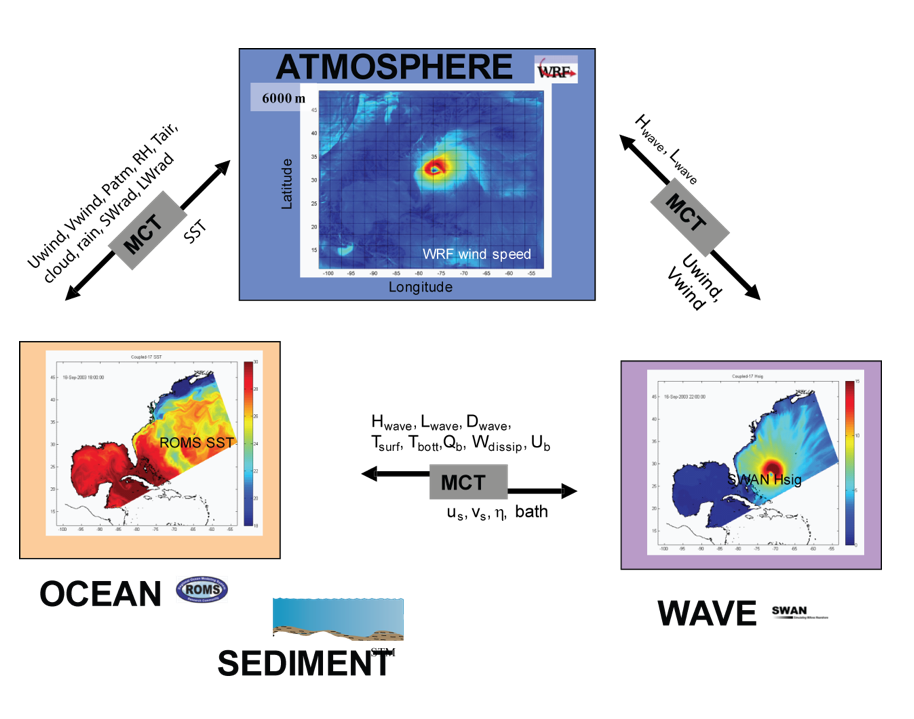
\includegraphics[width=0.55\textwidth]{model.png}
    \caption{Esquema que detalha a troca de informações entre os modelos que compõem o COAWST. \newline Fonte: \textcite{Warner2018}.}
    \label{acopla}
\end{figure}
\bigskip

\noindent A página do Woods Hole Coastal and Marine Science Center fornece, em caráter experimental, uma apresentação em tempo real da integração do COAWST (Temperatura da Superfície do Mar, Altura da Superfície do Mar, Altura Significativa de Ondas, Vetores de Corrente e Vento e dispersão de Sedimentos) para o leste dos Estados Unidos e Golfo do México. É possível acessar o conteúdo em \textcolor{bleu_cite}{\textit{https://woodshole.er.usgs.gov/project-pages/cccp/public/COAWST.htm}}.

%%%%%%%%%%%%%%%%%%%%%  PYTHON %%%%%%%%%%%%%%%%%%%%%%%%%%%
\section{O Python}\index{Python}
\bigskip

\noindent O Python é uma linguagem de programação poderosa, projetada com a filosofia de enfatizar a importância do esforço do programador sobre o esforço computacional. Prioriza a legibilidade do código sobre a velocidade ou expressividade.
\bigskip

\noindent A linguagem preza pela simplicidade e eficácia e possui uma ampla comunidade, o que facilita muito ao usuário em caso de dúvidas, pois encontra-se facilemnte através da internet um extenso acervo de bibliotecas e documentação.
\bigskip

\noindent O Python Brasil (\textcolor{bleu_cite}{\textit{http://python.org.br}}) oferece grande auxílio para iniciantes na linguagem, disponibilizando introduções (\textcolor{bleu_cite}{\textit{http://python.org.br/introducao/}}) e também um guia (\textcolor{bleu_cite}{\textit{http://python.org.br/cientifico}}) para usar o Python no meio científico.



%%%%%%%%%%%%%%%%%%%%%%%%%%% MATERIAIS %%%%%%%%%%%%%%%%%%%%%%%%%%%%%
\section{Materiais necessários para o uso do guia}\index{Materiais}
\bigskip

\noindent Este guia foi construído utilizando o elementary OS 0.4 Loki, baseado no Ubuntu 16.04 LTS. Esta versão conta com o gcc 5.4.0. Isso é importante pois versões diferentes podem gerar conflitos ao utilizar o pacote model2roms no próprio computador.
\bigskip

\noindent Este guia utiliza o COAWST v. 3.2. É importante manter a versão utilizada, pois versão diferentes podem apresentar problemas na compilação e integração.
